\documentclass{article}
\usepackage{xeCJK,amsmath,geometry,float,graphicx,amssymb,zhnumber,booktabs,setspace,tasks,verbatim,amsthm,amsfonts,mathdots}
\usepackage{listings,xcolor}
\geometry{a4paper,scale=0.8}   
\title{图论作业 (第五周)}
\author{PB20000113孔浩宇}
\begin{document}
\maketitle
\section*{Ch3}
\subsection*{3.}
\begin{proof}
    \begin{enumerate}
        \item []
        \item [(1)]$\delta (G)=\nu (G)-1 $,$\ G$为完全图,$\ \kappa (G)=\nu (G)-1 =\delta (G)$,成立.
        \item [(2)]$\delta (G)=\nu (G)-2 $.
        \begin{enumerate}
            \item [(a)]任意取$S\subseteq V,|S|=\nu(G)-3$,则
            \[
                \forall\ p\in G-S,\ d(p)\geq \nu (G)-2>\nu (G)-3\ 
                \Rightarrow\ 
                \exists\ q\in G-S,pq\in E(G-S).
            \]
            即$\kappa (G)\geq \nu (G) -2$.
            \item [(b)]$\delta (G)=\nu (G)-2\ \Rightarrow\ \exists\ p\in G,\ d(p)=\nu(G)-2$.取$S=\{v|\ pv\in E(G)\}$.
            \[
                \mbox{记}\ q=V(G)-S-p,\ G-S=G[\{p,q\}]\xrightarrow{pq\notin E(G)} G-S\mbox{不连通}.
            \]
        \end{enumerate}
        综合$(a)(b)$,可得$\kappa (G)=\nu(G)-2=\delta(G)$.
    \end{enumerate}
    综合$(1)(2)$,即证.
\end{proof}
\subsection*{7.}
\begin{proof}
    \begin{enumerate}
        \item []
        \item [(1)]$l=n$.即$l=m=n$,取$G=K_{n+1}$即可.
        \item [(2)]$l<n$.取$n+1$阶完全图$K_1,K_2$,取$K_1$中$l$个顶点记为$X$,$K_2$中$m$个顶点记为$Y$.
        \begin{enumerate}
            \item [(a)]取$Y$中$l$个顶点与$X$中顶点一一连线,$Y$中剩余$m-l$个顶点与$X$中顶点任意连接.
            \item [(b)]记$E=\{pq|\ p\in X,q\in Y\},G=K_1+K_2+E$.
        \end{enumerate}
        \[
            \begin{cases}
                l<n\ \Rightarrow \ \exists\ w\in G,d(w)=n &\Rightarrow\ \delta(G)\leq n\\
                \\
                K_1=K_2=K_{n+1}\ &\Rightarrow\ \delta(G)\geq n
            \end{cases}
            \ \Rightarrow\ 
            \delta(G)=n.
        \]
        \[
            \begin{cases}
                \{pq|\ p\in E(K_1)-X,\ q\in E(K_2)\}=\Phi\ \Rightarrow G-X\mbox{非连通}\ &\Rightarrow \kappa(G)=l\\
                \\
                \{pq|\ p\in E(K_1),\ q\in E(K_2),pq\notin E\}=\Phi\ \Rightarrow G-E\mbox{非连通}\ &\Rightarrow \kappa '(G)=m
            \end{cases}
        \]
        即证此时$G$满足要求.
    \end{enumerate}
    即证.
\end{proof}
\subsection*{11.}
\begin{proof}
    \begin{enumerate}
        \item []由$G$连通且不是块,可得$|G|\geq 3$.对$|G|$进行归纳.
        \item [(1)]$|G|=3$.如图,仅有一种情况,此时顶点导出子图$G[\{u,v\}]$与$G[\{w,v\}]$满足要求.
        \begin{figure}[H]
            \centering
            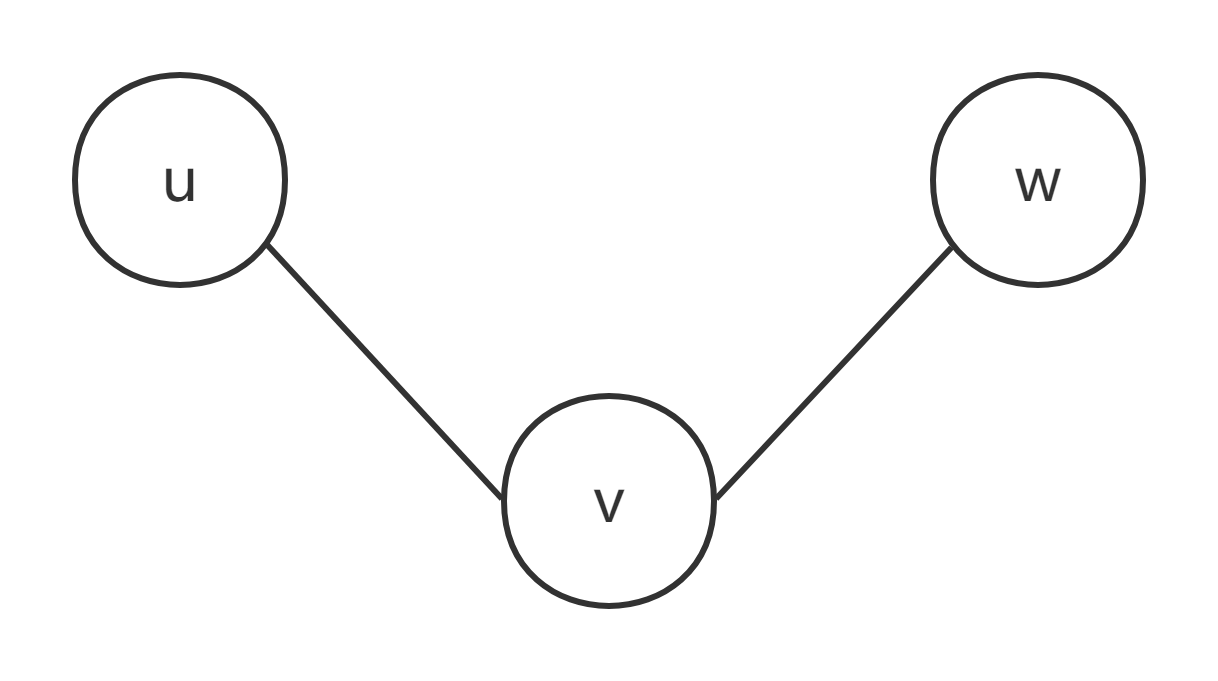
\includegraphics[scale=0.2]{1.png}
        \end{figure}
        \item [(2)]假设$|G|=n$时成立,考虑$|G|=n+1$.由$G$连通且不是块,可得$G$至少有一个割顶,记为$v$.
        
        由$v$为割顶可得$G-v$不连通,则$G-v$中至少有两个连通片,记为$G_1,G_2$.
        \begin{enumerate}
            \item [(a)]$G_1,G_2$均不含割顶.即$\kappa(G_1),\kappa(G_2)\geq 2$.记$V[G_1]\cup \{v\}=V_1$,$V[G_2]\cup \{v\}=V_2$.
            \[
                \begin{cases}
                    \kappa (G[V_1]) & =\kappa (G_1) \geq 2\\
                    \\
                    \kappa (G[V_2]) & =\kappa (G_2) \geq 2
                \end{cases}
                \ \Rightarrow\ 
                G[V_1],G[V_2] \mbox{为块,且每个仅含$G$的一个割顶}.
            \]
            此时命题成立.
            \item [(b)]若存在一个连通片$G_1$中含有割顶.
            \begin{enumerate}
                \item [$1^\circ$]由$|G_1|<|G-v|=n$,可得$G_1$中至少有两个块,每个块仅含一个$G_1$割顶.
                \item [$2^\circ$]记$G_1$的割顶为$u$,$G_1-u$不连通可得$G-u$不连通,即$G_1$的割顶也是$G$的割顶.
            \end{enumerate}\
            此时$G$中至少有两个块,每个块仅含$G$的一个割顶.
        \end{enumerate}
        即证$|G|=n+1$时命题成立.综上,$\forall\ |G|\geq 3$,原命题均成立.
    \end{enumerate}
\end{proof}
\subsection*{16.}
\begin{proof}
    假设存在图$G$,$G$的顶点度数均为偶数,且$G$中有桥,不妨设为$pq=e$.
    \begin{enumerate}
        \item [(0)]$e$为图$G$的桥$\Leftrightarrow$
        存在$V(G)$的一个划分$V(G)=U\cup W,\ U\cap W=\Phi,\ U,W\neq \Phi$,
        使得$\forall\ u\in U,w\in W$,$e$在每一条从$u$到$v$的轨道上.
        \item [(1)]先证明$p,q$不在同一个划分里.不妨设$p,q\in U$.
        
        $\forall\ w\in W,\ p$到$q$的轨道上含有$pq$,记为$p q W_{qw} w$,则$q,w$之间的轨道$W_{qw}$不含$pq$,矛盾.

        即证$p,q$在不同的划分中,不妨记$p\in U,\ q\in W$.
        \item [(2)]再证明$\{uw|\ u\in U, w\in W,uw\neq e\}=\Phi$.显然成立.
        \item [(3)]
        \[
            \sum\limits_{v\in U} \deg_{G[U]} (v)=\deg_{G} (p)-1+\sum\limits_{v\in U,v\neq q} \deg_{G} (v)
            \mbox{为奇数,矛盾}.
        \]
    \end{enumerate}
    假设不成立,即证若图$G$的顶点度数均为偶数,则$G$中没有桥.
\end{proof}
\end{document}

%\begin{align*}
%    \mbox{原式}
%    &= (1-z+z^2) \left[\sum\limits_{n=0}^{+\infty} \displaystyle{\frac{{(-1)}^n}{{(2n)}!}} z^{2n} \right]\\
%    &= (1-z+z^2) \left[\sum\limits_{n=0}^{+\infty} \displaystyle{\frac{\cos(\pi n)}{{(2n)}!}} z^{2n}\right]\\
%    &= (1-z+z^2) \left[\sum\limits_{n=0}^{+\infty} \displaystyle{\frac{\cos(\frac{\pi n}{2})}{{(n)}!}} z^n\right]\\
%    &= \left(\sum\limits_{n=0}^{+\infty} \displaystyle{\frac{\cos(\frac{\pi n}{2})}{{(n)}!}} z^n\right)
%    - \left(\sum\limits_{n=0}^{+\infty} \displaystyle{\frac{\cos(\frac{\pi n}{2})}{{(n)}!}} z^{n+1}\right)
%    +\left(\sum\limits_{n=0}^{+\infty} \displaystyle{\frac{\cos(\frac{\pi n}{2})}{{(n)}!}} z^{n+2}\right)\\
%    & =1+ \left(\sum\limits_{n=2}^{+\infty} \displaystyle{\frac{\cos(\frac{\pi n}{2})}{{(n)}!}} z^n\right)
%    - \left(\sum\limits_{n=1}^{+\infty} \displaystyle{\frac{\cos(\frac{\pi n}{2})}{{(n)}!}} z^{n+1}\right)
%    - z
%    +\left(\sum\limits_{n=0}^{+\infty} \displaystyle{\frac{\cos(\frac{\pi n}{2})}{{(n)}!}} z^{n+2}\right)\\
%    & = 1-z+\sum\limits_{n=0}^{+\infty} \displaystyle{\frac{\cos(\frac{n\pi+2\pi}{2}) - (n+2)\cos(\frac{n\pi+\pi}{2}) +(n+1)(n+2)\cos(\frac{n\pi}{2})}{(n+2)!}} z^{n+2}\\
%    & = 1-z+\sum\limits_{n=2}^{+\infty} \displaystyle{\frac{[n(n-1)-1]\cos(\frac{(n-2)\pi}{2})+n\sin\frac{(n-2)\pi}{2}}{n!}} z^n\\
%    & = \sum\limits_{n=0}^{+\infty}\displaystyle{\frac{(1+n-n^2)\cos\frac{n\pi}{2}-n\sin\frac{n\pi}{2}}{n!}} z^n
%\end{align*}